\documentclass[tikz,border=0pt]{standalone}
\usepackage{fontspec}
\hyphenpenalty=10000
\exhyphenpenalty=10000
\setmainfont[Path=../fonts/,BoldFont=Poppins-SemiBold.ttf,ItalicFont=Poppins-Italic.ttf]{Poppins-Regular.ttf}
\usepackage{pgfplots}
\pgfplotsset{compat=1.18}
\usetikzlibrary{calc,arrows.meta}
\definecolor{ink}{HTML}{161b22}
\definecolor{text}{HTML}{353535}
\definecolor{muted}{HTML}{646c74}
\definecolor{line}{HTML}{d7dadd}
\definecolor{wash}{HTML}{f6f6f6}
\definecolor{tint}{HTML}{e6ecef}
\definecolor{link}{HTML}{1d63b7}
\definecolor{local}{HTML}{376c97}
\definecolor{api}{HTML}{995d46}
\definecolor{cloud}{HTML}{7b649b}
\definecolor{match}{HTML}{7d9fc4}
\definecolor{miss}{HTML}{e0e3e5}
\begin{document}
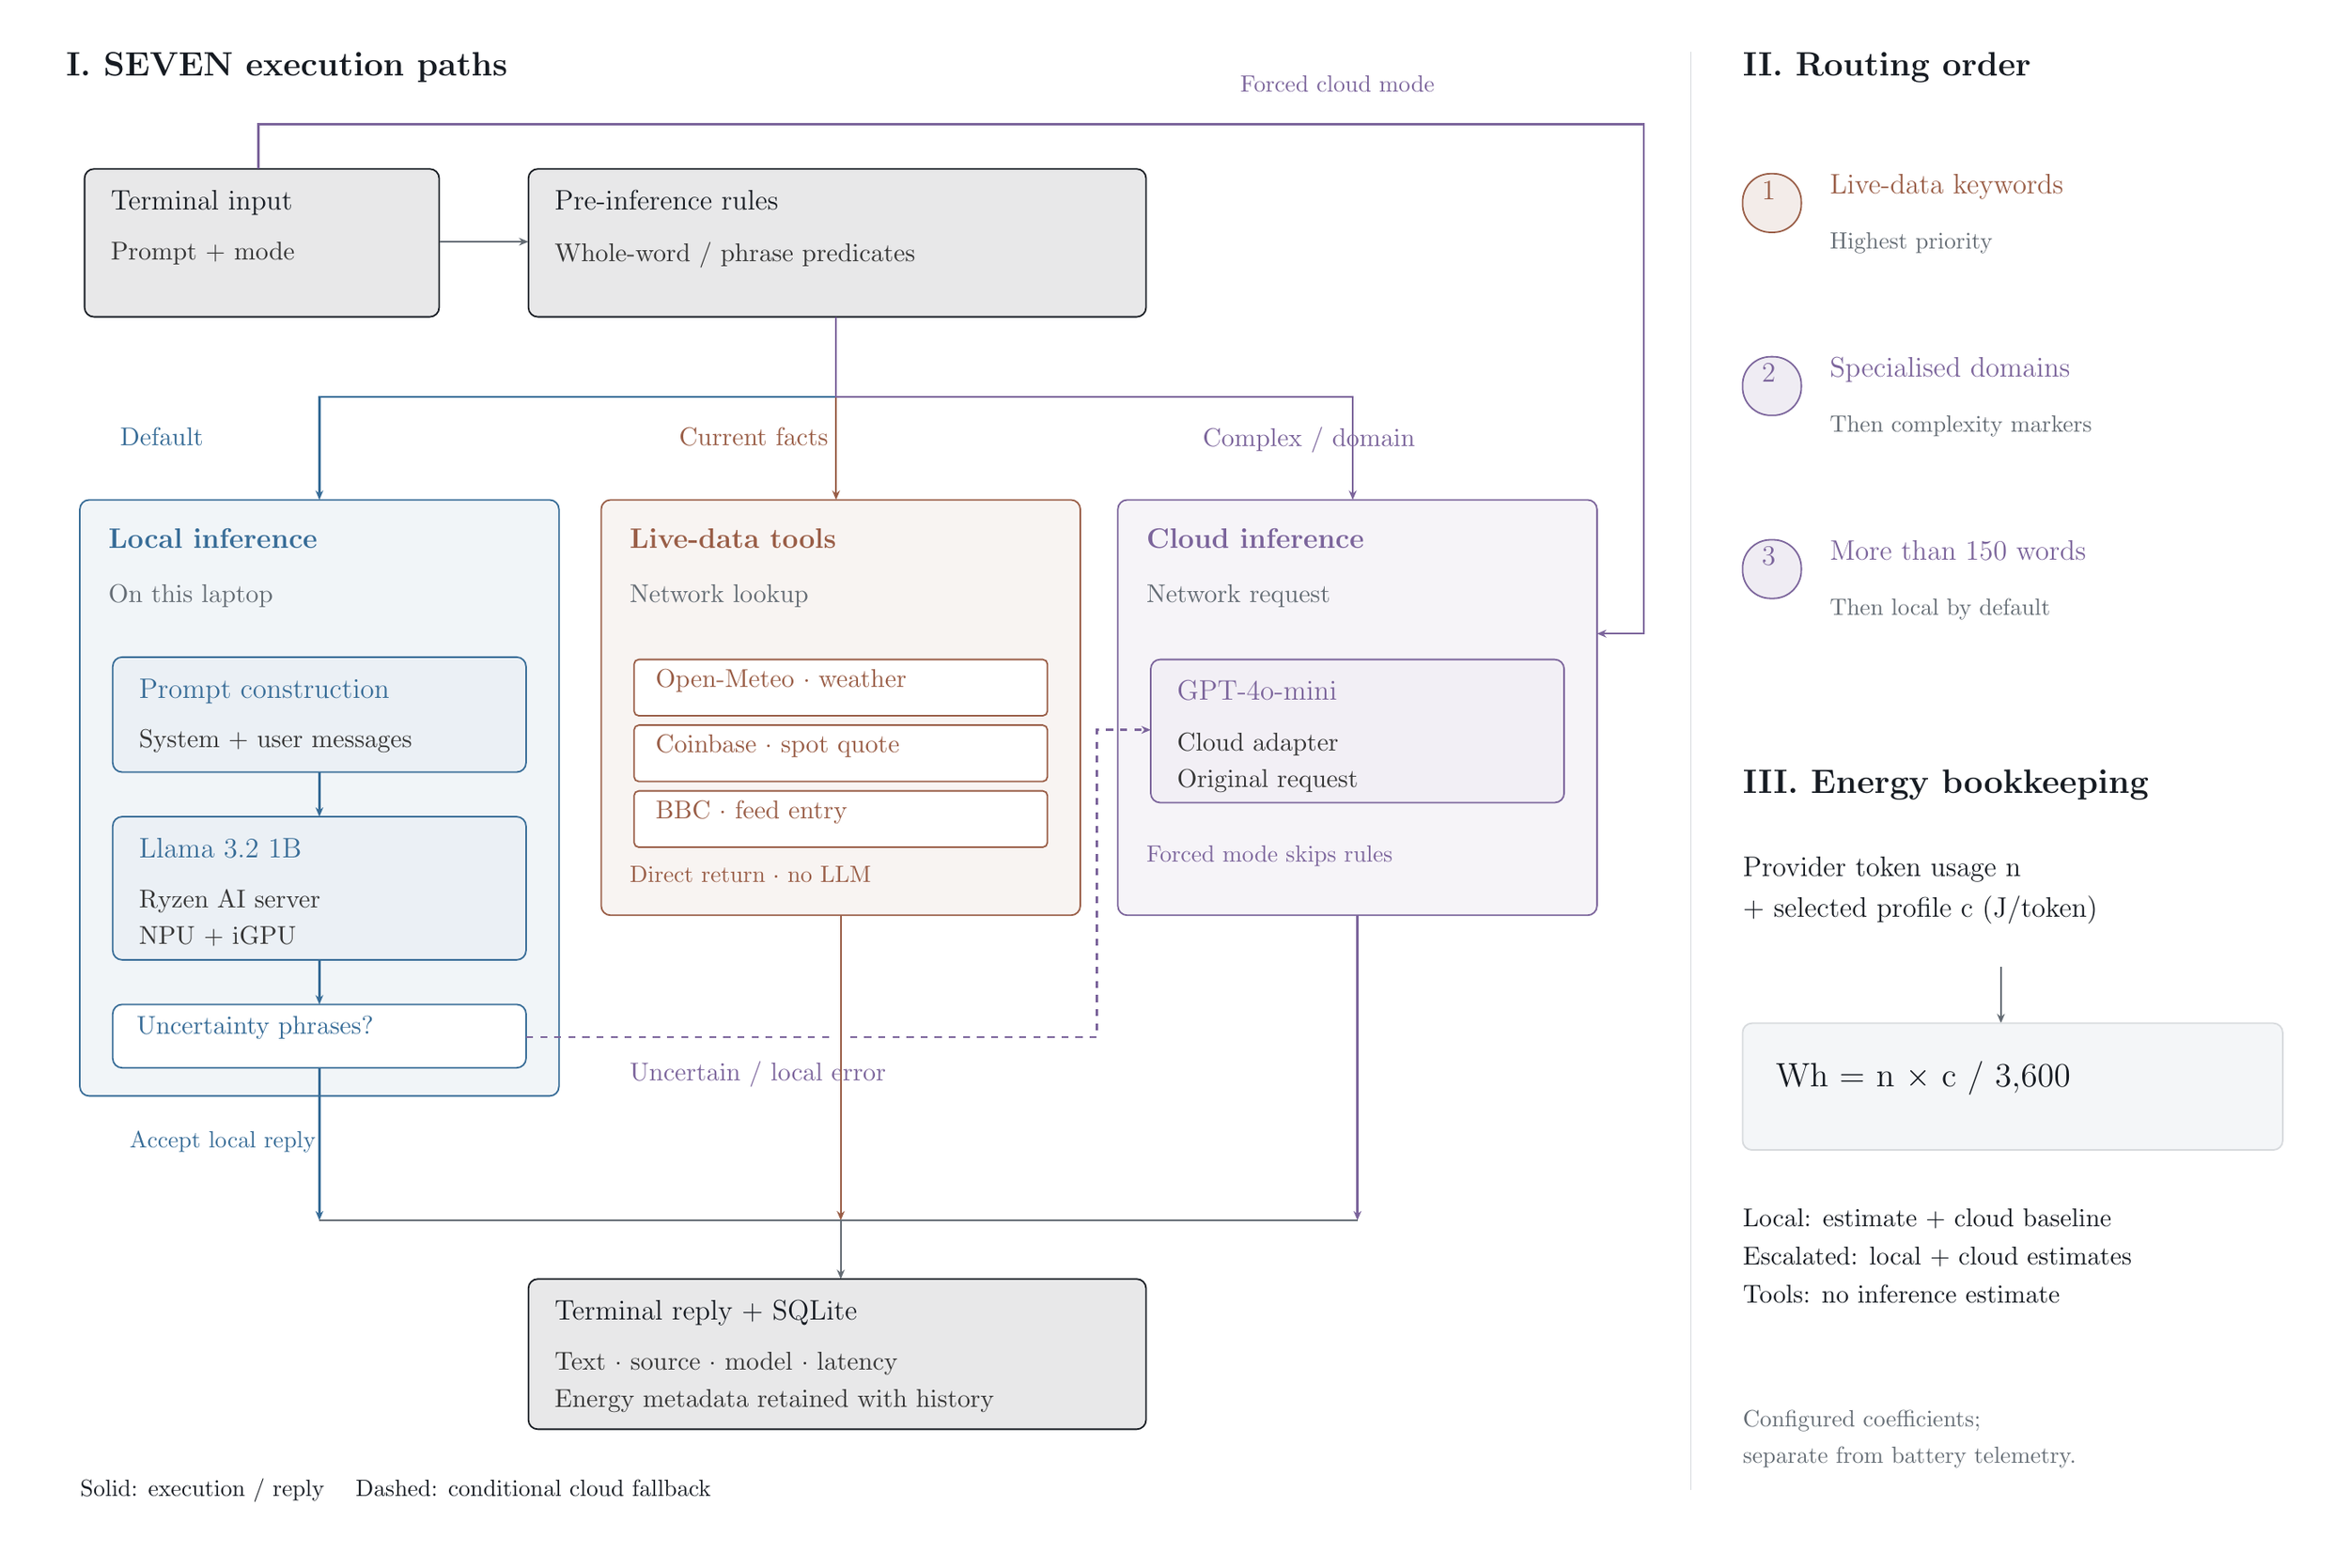
\begin{tikzpicture}[x=1pt,y=-1pt]
\path[use as bounding box] (0,0) rectangle (980,648);
\node[anchor=north west,inner sep=0pt,text=ink,align=left,font=\fontsize{14}{21.0}\selectfont] at (18,12) {\textbf{I. SEVEN execution paths}};
\node[anchor=north west,inner sep=0pt,text=ink,align=left,font=\fontsize{14}{21.0}\selectfont] at (732,12) {\textbf{II. Routing order}};
\draw[line,line width=.6pt] (710,12) -- (710,625);
\path[draw=ink,fill=ink!10!white,line width=.65pt,rounded corners=4pt] (26,62) rectangle (177,125);
\node[anchor=north west,inner sep=0pt,text=ink,align=left,font=\fontsize{12}{18.0}\selectfont] at (37,71) {Terminal input};
\node[anchor=north west,inner sep=0pt,text=text,align=left,font=\fontsize{10.5}{15.75}\selectfont,text width=129pt] at (37,93) {Prompt + mode};
\draw[-{Stealth[length=4pt,width=3.3pt]},line width=.85pt,draw=cloud] (100,62) -- (100,43) -- (690,43) -- (690,260) -- (670,260);
\node[anchor=north west,inner sep=0pt,text=cloud,align=left,font=\fontsize{10}{15.0}\selectfont] at (518,22) {Forced cloud mode};
\draw[-{Stealth[length=4pt,width=3.3pt]},line width=.85pt,draw=muted] (177,93) -- (215,93);
\path[draw=ink,fill=ink!10!white,line width=.65pt,rounded corners=4pt] (215,62) rectangle (478,125);
\node[anchor=north west,inner sep=0pt,text=ink,align=left,font=\fontsize{12}{18.0}\selectfont] at (226,71) {Pre-inference rules};
\node[anchor=north west,inner sep=0pt,text=text,align=left,font=\fontsize{10.5}{15.75}\selectfont,text width=241pt] at (226,93) {Whole-word / phrase predicates};
\draw[-{Stealth[length=4pt,width=3.3pt]},line width=.85pt,draw=local] (346,125) -- (346,159) -- (126,159) -- (126,203);
\draw[-{Stealth[length=4pt,width=3.3pt]},line width=.85pt,draw=api] (346,125) -- (346,203);
\draw[-{Stealth[length=4pt,width=3.3pt]},line width=.85pt,draw=cloud] (346,125) -- (346,159) -- (566,159) -- (566,203);
\node[anchor=north west,inner sep=0pt,text=local,align=left,font=\fontsize{11}{16.5}\selectfont] at (41,172) {Default};
\node[anchor=north west,inner sep=0pt,text=api,align=left,font=\fontsize{11}{16.5}\selectfont] at (279,172) {Current facts};
\node[anchor=north west,inner sep=0pt,text=cloud,align=left,font=\fontsize{11}{16.5}\selectfont] at (502,172) {Complex / domain};
\path[draw=local,fill=local!7!white,line width=.65pt,rounded corners=4pt] (24,203) rectangle (228,457);
\node[anchor=north west,inner sep=0pt,text=local,align=left,font=\fontsize{13}{19.5}\selectfont] at (36,215) {\textbf{Local inference}};
\node[anchor=north west,inner sep=0pt,text=muted,align=left,font=\fontsize{10.5}{15.75}\selectfont] at (36,239) {On this laptop};
\path[draw=local,fill=local!10!white,line width=.65pt,rounded corners=4pt] (38,270) rectangle (214,319);
\node[anchor=north west,inner sep=0pt,text=local,align=left,font=\fontsize{12}{18.0}\selectfont] at (49,279) {Prompt construction};
\node[anchor=north west,inner sep=0pt,text=text,align=left,font=\fontsize{10.5}{15.75}\selectfont,text width=154pt] at (49,301) {System + user messages};
\draw[-{Stealth[length=4pt,width=3.3pt]},line width=.85pt,draw=local] (126,319) -- (126,338);
\path[draw=local,fill=local!10!white,line width=.65pt,rounded corners=4pt] (38,338) rectangle (214,399);
\node[anchor=north west,inner sep=0pt,text=local,align=left,font=\fontsize{12}{18.0}\selectfont] at (49,347) {Llama 3.2 1B};
\node[anchor=north west,inner sep=0pt,text=text,align=left,font=\fontsize{10.5}{15.75}\selectfont,text width=154pt] at (49,369) {Ryzen AI server\\NPU + iGPU};
\draw[-{Stealth[length=4pt,width=3.3pt]},line width=.85pt,draw=local] (126,399) -- (126,418);
\path[draw=local,fill=white,line width=.65pt,rounded corners=4pt] (38,418) rectangle (214,445);
\node[anchor=north west,inner sep=0pt,text=local,align=left,font=\fontsize{11}{16.5}\selectfont] at (48,423) {Uncertainty phrases?};
\path[draw=api,fill=api!7!white,line width=.65pt,rounded corners=4pt] (246,203) rectangle (450,380);
\node[anchor=north west,inner sep=0pt,text=api,align=left,font=\fontsize{13}{19.5}\selectfont] at (258,215) {\textbf{Live-data tools}};
\node[anchor=north west,inner sep=0pt,text=muted,align=left,font=\fontsize{10.5}{15.75}\selectfont] at (258,239) {Network lookup};
\path[draw=api,fill=white,line width=.65pt,rounded corners=2pt] (260,271) rectangle (436,295);
\node[anchor=north west,inner sep=0pt,text=api,align=left,font=\fontsize{10.5}{15.75}\selectfont] at (269,275) {Open-Meteo · weather};
\path[draw=api,fill=white,line width=.65pt,rounded corners=2pt] (260,299) rectangle (436,323);
\node[anchor=north west,inner sep=0pt,text=api,align=left,font=\fontsize{10.5}{15.75}\selectfont] at (269,303) {Coinbase · spot quote};
\path[draw=api,fill=white,line width=.65pt,rounded corners=2pt] (260,327) rectangle (436,351);
\node[anchor=north west,inner sep=0pt,text=api,align=left,font=\fontsize{10.5}{15.75}\selectfont] at (269,331) {BBC · feed entry};
\node[anchor=north west,inner sep=0pt,text=api,align=left,font=\fontsize{10}{15.0}\selectfont] at (258,359) {Direct return · no LLM};
\path[draw=cloud,fill=cloud!7!white,line width=.65pt,rounded corners=4pt] (466,203) rectangle (670,380);
\node[anchor=north west,inner sep=0pt,text=cloud,align=left,font=\fontsize{13}{19.5}\selectfont] at (478,215) {\textbf{Cloud inference}};
\node[anchor=north west,inner sep=0pt,text=muted,align=left,font=\fontsize{10.5}{15.75}\selectfont] at (478,239) {Network request};
\path[draw=cloud,fill=cloud!10!white,line width=.65pt,rounded corners=4pt] (480,271) rectangle (656,332);
\node[anchor=north west,inner sep=0pt,text=cloud,align=left,font=\fontsize{12}{18.0}\selectfont] at (491,280) {GPT-4o-mini};
\node[anchor=north west,inner sep=0pt,text=text,align=left,font=\fontsize{10.5}{15.75}\selectfont,text width=154pt] at (491,302) {Cloud adapter\\Original request};
\node[anchor=north west,inner sep=0pt,text=cloud,align=left,font=\fontsize{10.2}{15.299999999999999}\selectfont] at (478,350) {Forced mode skips rules};
\draw[-{Stealth[length=4pt,width=3.3pt]},line width=.85pt,draw=cloud,dashed] (214,432) -- (457,432) -- (457,301) -- (480,301);
\node[anchor=north west,inner sep=0pt,text=cloud,align=left,font=\fontsize{10.5}{15.75}\selectfont] at (258,442) {Uncertain / local error};
\draw[-{Stealth[length=4pt,width=3.3pt]},line width=.85pt,draw=local] (126,445) -- (126,510);
\node[anchor=north west,inner sep=0pt,text=local,align=left,font=\fontsize{10}{15.0}\selectfont] at (45,472) {Accept local reply};
\draw[-{Stealth[length=4pt,width=3.3pt]},line width=.85pt,draw=api] (348,380) -- (348,510);
\draw[white,line width=4pt] (348,428) -- (348,436);
\draw[api,line width=.85pt] (348,428) -- (348,436);
\draw[-{Stealth[length=4pt,width=3.3pt]},line width=.85pt,draw=cloud] (568,380) -- (568,510);
\draw[muted,line width=.8pt] (126,510) -- (568,510);
\draw[-{Stealth[length=4pt,width=3.3pt]},line width=.85pt,draw=muted] (348,510) -- (348,535);
\path[draw=ink,fill=ink!10!white,line width=.65pt,rounded corners=4pt] (215,535) rectangle (478,599);
\node[anchor=north west,inner sep=0pt,text=ink,align=left,font=\fontsize{12}{18.0}\selectfont] at (226,544) {Terminal reply + SQLite};
\node[anchor=north west,inner sep=0pt,text=text,align=left,font=\fontsize{10.5}{15.75}\selectfont,text width=241pt] at (226,566) {Text · source · model · latency\\Energy metadata retained with history};
\node[anchor=north west,inner sep=0pt,text=ink,align=left,font=\fontsize{10}{15.0}\selectfont] at (24,620) {Solid: execution / reply \quad Dashed: conditional cloud fallback};
\path[draw=api,fill=api!12!white,line width=.65pt,rounded corners=12pt] (732,64) rectangle (757,89);
\node[anchor=north west,inner sep=0pt,text=api,align=left,font=\fontsize{12}{18.0}\selectfont] at (740,67) {1};
\node[anchor=north west,inner sep=0pt,text=api,align=left,font=\fontsize{12}{18.0}\selectfont] at (769,64) {Live-data keywords};
\node[anchor=north west,inner sep=0pt,text=muted,align=left,font=\fontsize{10.2}{15.299999999999999}\selectfont] at (769,89) {Highest priority};
\path[draw=cloud,fill=cloud!12!white,line width=.65pt,rounded corners=12pt] (732,142) rectangle (757,167);
\node[anchor=north west,inner sep=0pt,text=cloud,align=left,font=\fontsize{12}{18.0}\selectfont] at (740,145) {2};
\node[anchor=north west,inner sep=0pt,text=cloud,align=left,font=\fontsize{12}{18.0}\selectfont] at (769,142) {Specialised domains};
\node[anchor=north west,inner sep=0pt,text=muted,align=left,font=\fontsize{10.2}{15.299999999999999}\selectfont] at (769,167) {Then complexity markers};
\path[draw=cloud,fill=cloud!12!white,line width=.65pt,rounded corners=12pt] (732,220) rectangle (757,245);
\node[anchor=north west,inner sep=0pt,text=cloud,align=left,font=\fontsize{12}{18.0}\selectfont] at (740,223) {3};
\node[anchor=north west,inner sep=0pt,text=cloud,align=left,font=\fontsize{12}{18.0}\selectfont] at (769,220) {More than 150 words};
\node[anchor=north west,inner sep=0pt,text=muted,align=left,font=\fontsize{10.2}{15.299999999999999}\selectfont] at (769,245) {Then local by default};
\node[anchor=north west,inner sep=0pt,text=ink,align=left,font=\fontsize{14}{21.0}\selectfont] at (732,318) {\textbf{III. Energy bookkeeping}};
\node[anchor=north west,inner sep=0pt,text=ink,align=left,font=\fontsize{11.5}{17.25}\selectfont] at (732,355) {Provider token usage n\\+ selected profile c (J/token)};
\draw[-{Stealth[length=4pt,width=3.3pt]},line width=.85pt,draw=muted] (842,402) -- (842,426);
\path[draw=line,fill=tint!45!white,line width=.65pt,rounded corners=4pt] (732,426) rectangle (962,480);
\node[anchor=north west,inner sep=0pt,text=ink,align=left,font=\fontsize{15}{22.5}\selectfont] at (746,442) {Wh = n × c / 3,600};
\node[anchor=north west,inner sep=0pt,text=ink,align=left,font=\fontsize{10.8}{16.200000000000003}\selectfont] at (732,505) {Local: estimate + cloud baseline\\Escalated: local + cloud estimates\\Tools: no inference estimate};
\node[anchor=north west,inner sep=0pt,text=muted,align=left,font=\fontsize{10.2}{15.299999999999999}\selectfont] at (732,591) {Configured coefficients;\\separate from battery telemetry.};

\end{tikzpicture}
\end{document}
